\author{Matthias Hüning}\institute[FU Berlin, Philosophie und Geisteswissenschaften, Niederlandistik]{}

\subtitle{Überblick über die germanischen Sprachen}

\section{Überblick über die germanischen Sprachen}

\huberlintitlepage[22pt]


\outline{

\begin{itemize}
\item {Überblick über die germanischen Sprachen}
\item Phänomene
\item Phrasenstrukturgrammatiken und \xbart
\item Valenz, Argumentanordnung und Adjunkte
\item Verbalkomplexbildung in den SOV-Sprachen
\item Verbstellung: Verberst- und Verbzweitstellung
\item Passiv
\item Eingebettete Sätze
\end{itemize}

}

\frame{
\frametitle{Literaturhinweis}



Zu diesem Abschnitt gibt es das Kapitel~1 in \citew{MuellerGermanic}.


\begin{refsection}

\nocite{MuellerGermanic}

\printbibliography[heading=none,notkeyword=this]

\end{refsection}



}


%\part{Allgemeines}


\subsection{Sprachen und Sprecher*innen}

\frame{
\frametitle{Allgemeines: Sprachen und Sprecher*innen}


\begin{itemize}
\item ca.\ 5000 bis 6000 Sprachen auf der Welt
\pause
\item Germanische Sprachen bilden eine kleine Gruppe\\
(je nach Zählung etwa 15 Sprachen)
\pause
\item Problem: Abgrenzung von Sprache und Sprachvarietät\\
      (\zb Varietäten des Friesischen)\\
"`Eine Sprache ist ein Dialekt mit einer Armee und Flotte."' (Max Weinreich)
\pause
\item insgesamt fast 500 Millionen Sprecher*innen (Muttersprachler)\\
      $>$ 1/12 der Weltbevölkerung
\pause
\item große regionale Verbreitung (insbesondere Englisch)

\end{itemize}

}


\subsection{Gängige Einteilung}

\frame{
\frametitle{Gängige Einteilung}

\begin{itemize}
\item Ostgermanisch\\
Gotisch (ausgestorben)
\pause
\item Westgermanisch\\
Deutsch, Jiddisch, Luxemburgisch, Pennsylvanisch,
Plautdietsch, Niederländisch, Afrikaans, Friesisch, Englisch
\pause
\item Nordgermanisch\\
Dänisch, Schwedisch, Norwegisch, Isländisch, Färöisch
\end{itemize}


}

\subsection{Historische Bemerkungen}

\frame{
\begin{itemize}
\item Germanisch: selbständiger Zweig in der indoeuropäischen Sprachfamilie
\pause
\item Zwischen 2000 und 1000 v.\,Chr. Ausgliederung des Proto-Germanischen aus dem indoeuropäischen Sprachkontinuum
\pause
\item Ursprünge in der baltischen Region (Norddeutschland,
Südskandinavien); Ausbreitung von Nordsee bis Polen (ca.\,500
v.\,Chr.)
\pause
\item Veränderungen im Konsonantismus\\
      (Erste bzw. Germanische Lautverschiebung; bis ca.\ 2.\,Jh.\,v.\,Chr.)
\pause
\item Erste schriftliche Zeugnisse:\\
      Runeninschriften (ab ca.\ 300 n.\,Chr.; gotische Bibelübersetzung im 4.\,Jh.)
\end{itemize}

}


\subsection{Die indoeuropäische Sprachfamilie}


\frame{
\includegraphics[width=70mm]{Bilder/indoeuropaeisch}
aus \citew[S.\,665]{Fitch2007a-u}

}

\subsection{Verwandschaft}

\frame{
Lautliche Übereinstimmung bei Wörtern aus dem zentralen
Wortschatz

\oneline{%
\begin{tabular}{lllllllll}
Niederländisch & vader  & vier    & vol    & huis  & bruin  & uit & kruid     & muis\\
Deutsch        & Vater  & vier    & voll   & Haus  & braun  & aus & Kraut     & Maus\\
Englisch       & father & four    & full   & house & brown  & out & crowd (?) & mouse\\
Friesisch      & –      & fjouwer & fol    & hûs   & brún   & út  & krûd      & mûs\\
Schwedisch     & fader  & fyra    & full   & hus   & brun   & ut  & krut      & mus\\
Dänisch        & fader  & fire    & fuld   & hus   & brun   & ud  & krudt     & mus\\
Norwegisch     & far    & fire    & full   & hus   & brun   & ut  & krydder   & mus\\
Isländisch     & faðir  & fjórir  & fullur & hús   & brúnn  & út  & –         & mús\\
\end{tabular}
}

}

\subsection{Entwicklung der germanischen Sprachen}

\frame{
\frametitle{Entwicklung der germanischen Sprachen}


%\includegraphics[width=\textwidth]{Bilder/stammbaum-germanisch}
%aus \citew[S.\,251]{Bussmann2002a}


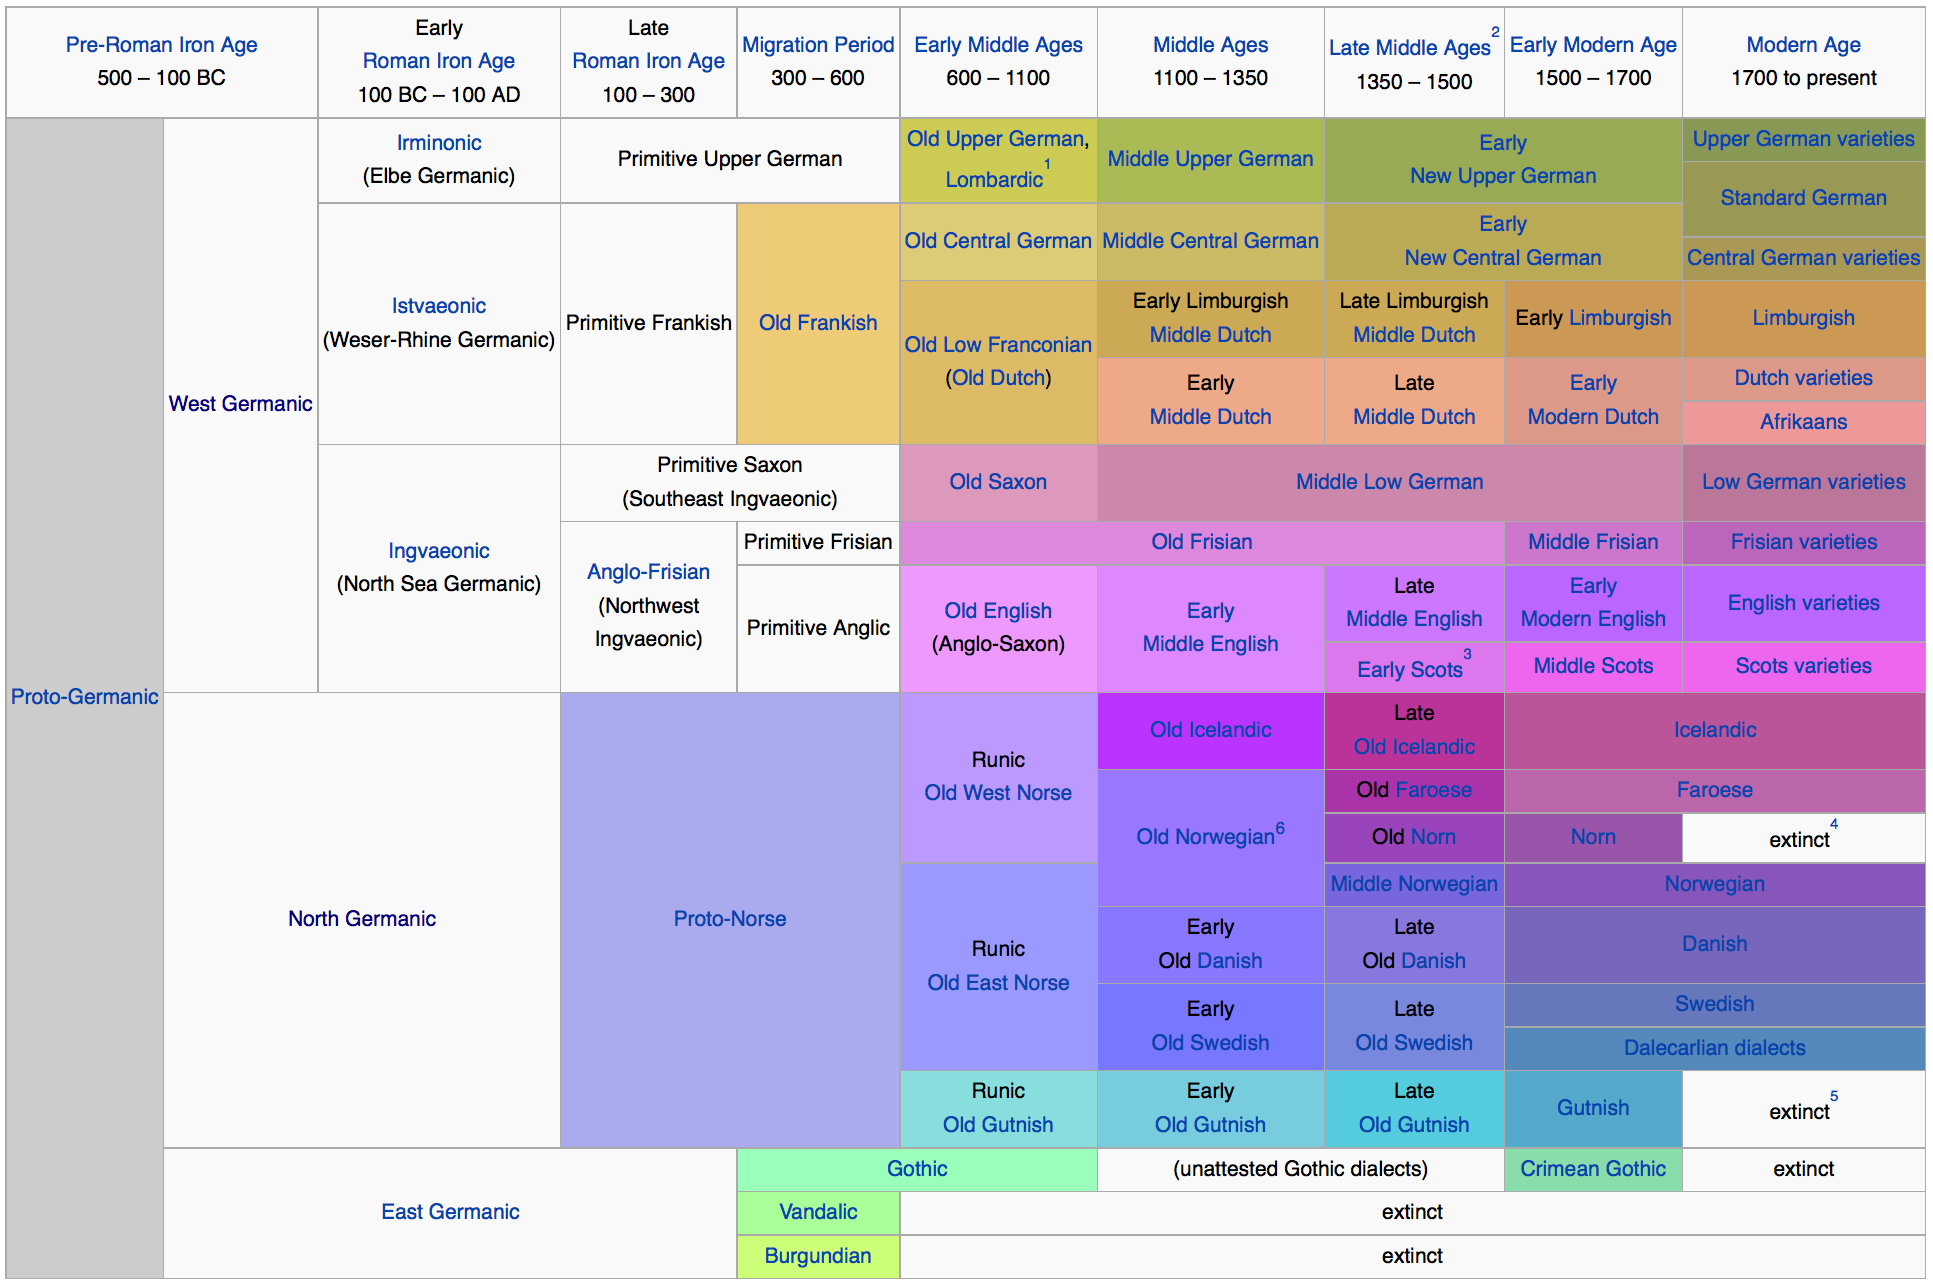
\includegraphics[width=.75\textwidth]{Bilder/germanic-wikipedia}

\oneline{Quelle: Englische Wikipedia: \url{https://en.wikipedia.org/wiki/Germanic_languages\#Diachronic}}


}



\subsection{Drei Zweige des Germanischen}

\frame{
\frametitle{Drei Zweige des Germanischen}

\begin{itemize}
\item Aufteilung des Protogermanischen in drei Zweige:\\
Ost-, West- und Nordgermanisch (etwa im ersten Jh.\ nach Chr.)
\pause

\item Ursachen:
\begin{itemize}
\item inhärente sprachliche Variation (Dialekte)
\item Migration (Sprachkontakt)
\item Standardisierung
\end{itemize}

\pause

\item Wir behandeln die Struktur germanischer Standardsprachen
\end{itemize}

}

\subsubsection{Ostgermanisch}

\frame{
\frametitle{Ostgermanisch}

\begin{itemize}
\item
ca.\ 100 v. Chr: Goten emigrieren von den dänischen Inseln
und aus Südschweden und treffen auf Vandalen und andere
Stämme
\pause
\item Sie konstituieren den ostgermanischen Zweig,\\ von dem nur
das Gotische überliefert ist
\pause
\item Mit dem Ende der Gotenreiche ist auch das Gotische
ausgestorben\\
(letzte Reste bis ca.\ 1800 auf der Halbinsel Krim)
\pause
\item Im 4.\ Jahrhundert übersetzte der westgotische Bischof
Wulfila die Bibel ins Gotische (Wulfila-Bibel)
\pause
\item  Bekannt ist vor allem das Manuskriptfragment in der
Universitätsbibliothek von Uppsala (Codex Argenteus)
\end{itemize}


}


\frame{
\frametitle{Wulfila-Bibel (Codex Argenteus)}

\begin{columns}[T]
\begin{column}{53mm}
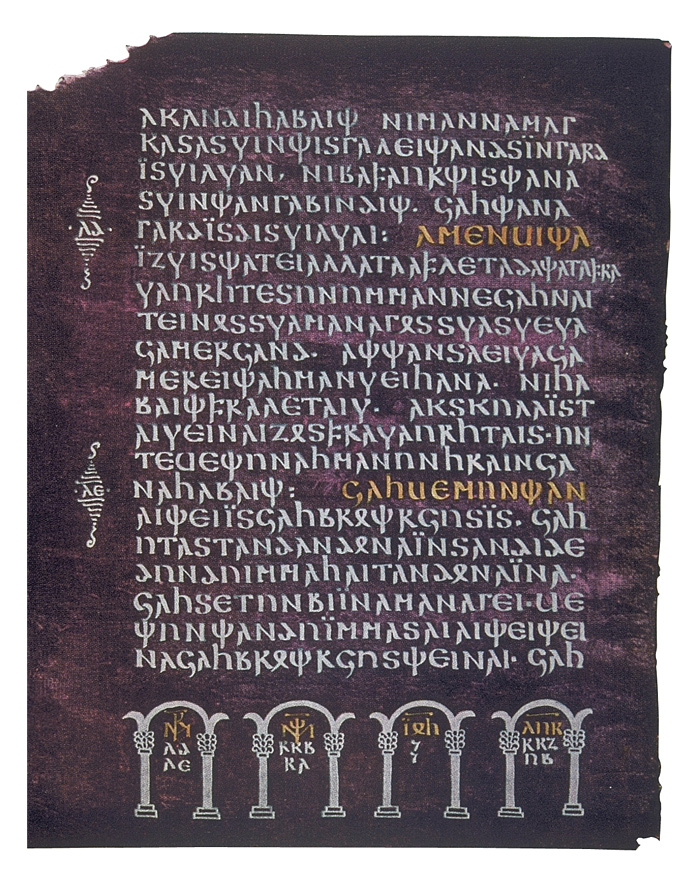
\includegraphics[width=53mm]{Bilder/Wulfila_bibel}
\end{column}
\begin{column}{65mm}

Quelle: Wikipedia\\
\url{http://de.wikipedia.org/wiki/Bild:Wulfila_bibel.jpg}
\end{column}
\end{columns}

}

\subsubsection{Nordgermanisch}

\frame{
\frametitle{Nordgermanisch}

\begin{itemize}
\item erste Runen-Inschriften aus dem 6.\,Jh.
\item Sprache der Wikinger (800--1050) war noch relativ homogen
\item erst gegen Ende der Wikinger-Ära entstanden zwei Zweige:\\
 Ost-Skandinavisch (Altdänisch, Altschwedisch),\\
 West-Skandinavisch (Altnorwegisch, Altisländisch)
\end{itemize}

}



\subsubsubsection{Dänisch}

\frame{
\frametitle{Dänisch}

\begin{itemize}
\item Dänisch (dansk): offizielle Sprache des Königreichs Dänemark,
zweite Amtssprache der Färöer-Inseln und Grönlands (Inuit als
erste Sprache)
\item ca.\ 5,5 Millionen Sprecher*innen
\item ca.\ 50.000 Sprecher*innen in Schleswig Holstein
\item das Dänische hat sich von allen skandinavischen Sprachen am
weitesten von den gemeinskandinavischen Wurzeln entfernt
\end{itemize}

}



\subsubsubsection{Schwedisch}

\frame{
\frametitle{Schwedisch}

\begin{itemize}
\item Schwedisch (svenska):\\
offizielle Sprache in Schweden mit ca.\ 8,5 Millionen Muttersprachlern
\item erste Sprache von ca.\ 300.000 Sprecher*innenn in Finnland
\item Bis zur Wikingerzeit sind Dänisch und Schwedisch kaum
voneinander zu unterscheiden; 

ab ca.\ 800 entwickeln sie sich auseinander; 

seit ca.\ 1300 deutlich unterscheidbar
\end{itemize}

}


\subsubsubsection{Isländisch}

\frame{
\frametitle{Isländisch}

\begin{itemize}
\item Isländisch (íslenska) ist die westskandinavische Sprache Islands
seit der Besiedlung vor über 1000 Jahren
\item ca.\ 260.000 Sprecher*innen
\item kaum Variation (keine Dialekte)
\item Konservativ: von allen skandinavischen Sprachen hat das
Isländische die Flexion und seinen germanischen Erbwortschatz
am besten bewahrt.
\item Zunächst kaum Unterschiede zum Norwegischen,\\
dann auseinander entwickelt
\end{itemize}

}



\subsubsubsection{Norwegisch}


\frame{
\frametitle{Norwegisch}

\begin{itemize}
\item Norwegisch (norsk) kennt zwei Varietäten:\\
Dänisch-Norwegisch (bokmål) und Neu-Norwegisch (nynorsk). 

Beide sind offizielle Landessprachen und werden nebeneinander verwendet.
\item Insgesamt ca.\ 4,3 Millionen Sprecher*innen.
\item Von 1380--1814 war Dänisch die Schriftsprache;\\
gesprochen wurden lokale Dialekte
\item norwegischer Standard musste daher erst geschaffen werden;\\
Ivar Aasen (1813--1896): nynorsk; offiziell anerkannt 1885
\item bokmål (`Buchsprache') ist die erste Sprache der Mehrheit
\end{itemize}

}




\subsubsubsection{Färöisch}

\frame{
\frametitle{Färöisch}

\begin{itemize}
\item Färöisch oder Färingisch (føroyskt) ist, zusammen mit Dänisch,\\
die offizielle Sprache der Färöer-Inseln
\item 47.000 Sprecher*innen
\item Färöer-Inseln gehören seit 1816 zu Dänemark, \\
seit 1948 Status eines autonomen Landesteils
\item Färöisch ist stark vom Dänischen beeinflusst
\item Schriftsprachliche Überlieferung erst seit 1773 und auch dann nur spärlich\\
(dies im Gegensatz zum Isländischen)
\end{itemize}

}




\subsubsection{Westgermanisch}

\frame{
\frametitle{Westgermanisch}

\begin{itemize}
\item kein homogener Ursprung, sondern drei Zweige von
Dialektgruppen (Nordseegermanisch, Weser-Rheingermanisch,
Elbgermanisch)
\item aber keine 1-zu-1-Zuordnung dieser Dialektgruppen zu den
heutigen Standardsprachen
\end{itemize}

}




\subsubsubsection{Deutsch}

\author{Matthias Hüning, Stefan Müller}\institute[FU Berlin, Philosophie und Geisteswissenschaften]{}

\frame{
\frametitle{Deutsch}


\begin{itemize}
\item Deutsch ist offizielle Landessprache von 
\begin{itemize}
\item Deutschland (ca.\ 80 Millionen Sprecher*innen), 
\item Österreich (7,5 Millionen), 
\item Liechtenstein
(15.000), 
\item Schweiz (4,2 Millionen, von insgesamt 6,4 Millionen
Schweizern), 
\item Italien/Südtirol (270.000), 
\item Belgien (65.000),
\item Luxemburg (360.000).
\end{itemize}
\item In Luxemburg gilt neben dem nicht-ursprünglichen Deutsch auch
das ursprüngliche Lëtzebuergesch als offizielle Sprache.
\item Insgesamt hat das Deutsche ca.\ 97 Millionen Sprecher*innen, davon
ca.\ 90 Millionen Muttersprachler und 7 Millionen
Zweitsprachler (täglicher Gebrauch)
% = Migrationshintergrund
% Quelle Wikipedia 15.10.2013


\item ca.\ 80 Mio Fremdsprachler, davon ca. 55 Mio in der EU
\end{itemize}

}




\author{Matthias Hüning}\institute[FU Berlin, Philosophie und Geisteswissenschaften, Niederlandistik]{}


\frame{
\frametitle{Deutsch}

\begin{itemize}
\item Drei nationale Hauptvarianten (Deutschland, Österreich, Schweiz);\\
in anderen Staaten meist Minderheitensprache
\item Zwei Dialektgruppen: Niederdeutsch/Plattdeutsch und
Hochdeutsch
\end{itemize}

}



\subsubsubsection{Jiddisch}

\frame{
\frametitle{Jiddisch}

\begin{itemize}
\item Jiddisch ist eine von vielen jüdischen Sprachen.\\
heute von ca.\ 2 Millionen Menschen in verschiedenen Regionen der Welt gesprochen,\\
davon die meisten in den USA (1,25 Mill.)
\item Vor 100 Jahren lebten weit über 7 Millionen Sprecher*innen des
Jiddischen in Europa, die meisten in Russland und in Österreich-Ungarn.
\item Heute höchstens noch 75.000 Jiddisch-Sprachige in Westeuropa
\item Ursprung: mittelalterliches Deutsch, vermischt mit Hebräisch und
Aramäisch
\end{itemize}

}


\subsubsubsection{Pennsylvania German}

\frame{
\frametitle{Pennsylvania German}

\begin{itemize}
\item Pennsylvanisch (Deitsch, auch bekannt als Pennsylvanian Dutch)
hat ca.\ 300.000 Muttersprachler, vor allem in den USA
\item Sprachinseln, vor allem in Pennsylvania, Ohio und Indiana
\item Auswanderung im 17. und 18. Jahrhundert; Mitglieder
verschiedener protestantischer Glaubensrichtungen (Mennoniten,
Pietisten usw.)
\item Sprache baut hauptsächlich auf Pfälzer Dialekten auf
\item heute vor allem gesprochen von Amischen und Mennoniten
\end{itemize}

}



\subsubsubsection{Niederländisch}

\frame{
\frametitle{Niederländisch}

\begin{itemize}
\item Niederländisch (Nederlands) ist offizielle Landessprache in den Niederlanden\\
(ca.\ 15 Millionen Sprecher*innen),\\
eine der Landessprachen in Belgien (ca.\ 6 Millionen; knapp 4 Millionen
Wallonen).
\item Es ist die offizielle Verwaltungs- und Unterrichtssprache in Surinam\\
 (seit 1975 unabhängig) und auf Aruba und den niederländischen Antillen
\end{itemize}

}



\subsubsubsection{Afrikaans}

\frame{
\frametitle{Afrikaans}

\begin{itemize}
\item Afrikaans ist eine der offiziellen Sprachen Südafrikas\\
      (insgesamt über 10 Amtssprachen)
\item ca.\ 6,4 Millionen Muttersprachler,
davon 6,2 Millionen in Südafrika\\ (= ca.\ 15\,\% der Bevölkerung) und 150.000 in Namibia
\item seit Mitte des 17.\ Jh.; Entwicklung aus niederländischen Dialekten;\\
Afrikaans wird seit dem frühen 19.\ Jh. als
eigenständige Sprache gesehen
\item Sprachkontakt; heute starker Einfluss des Englischen
\item starke Tendenzen zu struktureller Vereinfachung im
Sprachsystem
\end{itemize}

}



\subsubsubsection{Friesisch}

\frame{
\frametitle{Friesisch}

Drei Varietäten, untereinander nicht verständlich:\begin{itemize}
\item Nordfriesisch, ca.\ 10.000 Sprecher*innen, vor allem auf den
nordfriesischen Inseln (Amrum, Sylt, Helgoland)
\item Ostfriesisch, in Ostfriesland ausgestorben.\\
Überbleibsel: das Saterfriesische (wird in der Gemeinde Saterland im Landkreis
Cloppenburg von etwa 1.000 bis 2.500 Menschen
gesprochen)
\item Westfriesisch, niederländische Provinz Friesland,\\
 ca.\ 350.000 Muttersprachler
\end{itemize}


}



\subsubsubsection{Englisch}

\frame{
\frametitle{Englisch}

\begin{itemize}
\item Englisch hat gegen Ende des 20.\ Jh. ca.\ 570 Millionen Sprecher*innen in
aller Welt (337 Mill. Muttersprachler, 235 Mill. Zweitsprachler)
\begin{itemize}
\item USA: 227 Mill. Muttersprachler; 
\item Großbritannien: 57 Mill.;
\item Nigeria: 43 Mill.; 
\item Kanada: 24 Mill.; 
\item Australien: 17 Mill.; 
\item Irland: 3,5 Mill.; 
\item Neuseeland: 3,2 Mill.
\end{itemize}
\item Viele nationale Varianten (vor allem Aussprache)
\item Geschätzte 1 bis 1,5 Milliarden Menschen besitzen aktive oder
passive Englischkenntnisse
\item Amtlicher Status in 59 Staaten
\item Weltweit wichtigste Wissenschaftssprache
\end{itemize}

\pause\pause\pause
}

